\section{BaM}
\label{sec:chapter_4_section_1}
Il Progetto BaM (Building and Modelling), sviluppato in collaborazione con il CNG (Comitato Nazionale Geometri),
facente parte del progetto nazionale \emph{Georientiamoci}, per l’orientamento nella scelta
del percorso di studi degli studenti, per il passaggio tra le scuole medie e le superiori.
Questo progetto nasce dall'idea di far realizzare, agli studendi frequentanti le scuole medie in Italia,
``\emph{l'aula che vorrei}''. Questa iniziativa si prefigge di sensibilizzare gli studenti nell’u-
tilizzo di materiali ecosostenibili e rispettare l’ambiente.
Gli alunni avranno poi la possibilità di modellare un aula scegliendo gli elementi con cui personalizzare l’aula virtuale.
La lista degli oggetti 3D presenti in libreria ha l’obiettivo di far sperimentare l’uso di uno strumento di progettazione
e di rappresentazione della realtà e di dare spunti su alcune tematiche come:
\begin{itemize}
\item impatto Ecologico;
\item impatto Energetico;
\item sicurezza;
\item rispetto della diversità/disabilità;
\end{itemize}
Per questo motivo il framework \emph{Metior} è stato strutturato in modo che a ogni elemento sia associato un punteggio seguendo
la categorizzazione precedentemente definita.
Gli alunni suddivisi in gruppi un volta terminata la modellazione dell'aula, salveranno il loro modello che sarà valutato
dal framework.
Vincerà il gruppo che avra realizzato la classe con il punteggio più alto, risultante dalla somma dei materiali scelti
tra quelli presenti in libreria. Per ottenere un punteggio alto bisogna rispettare i principi delle
“3E” (Edilizia – Energia - Economia) e delle “3R” (Ridurre, Riutilizzare, Riciclare). In Figura \ref{fig:3daula} è presente
un modello di aula realizzato con il framework \emph{Metior}.\\
\begin{figure}[htbp] %  figure placement: here, top, bottom, or page
   \centering
   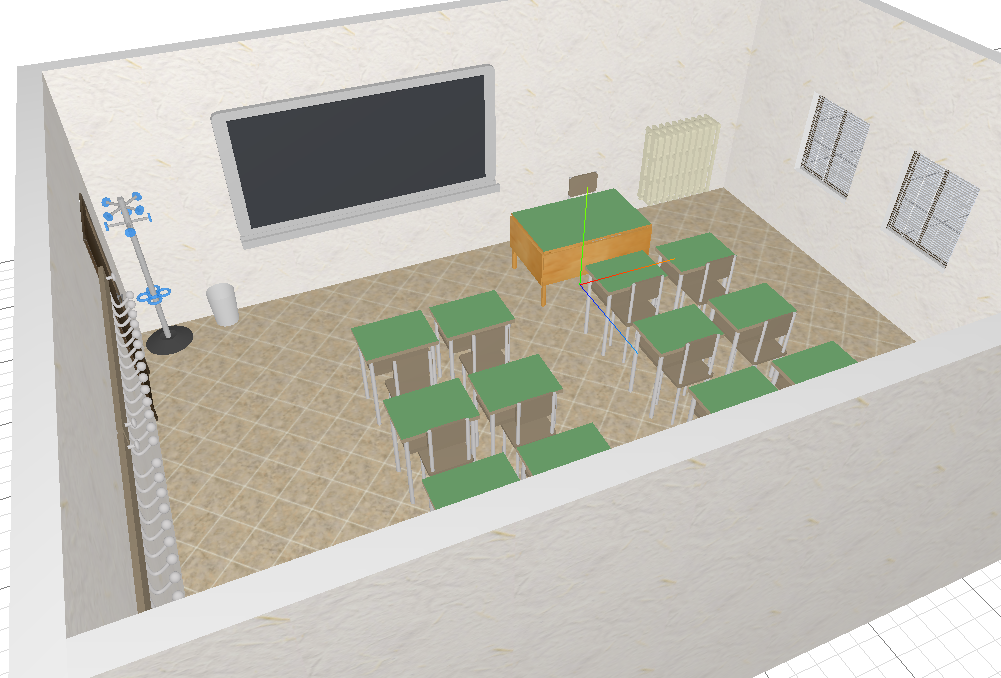
\includegraphics[width=0.6\linewidth]{images/3d-school-2}
   \caption{Vista 3D del modello di un'aula}
   \label{fig:3daula}
   \end{figure}
\newpage

Come descritto in precedenza i \emph{Plugin} presenti all'interno del catalogo sono stati suddivisi in categorie per
consentire una valutazione del modello di un'aula al termine dell'esperienza da parte degli studenti.
Il primo gruppo di \emph{Plugin} riportato sono (Figura~\ref{fig:figura1}): un appendiabiti, un armadietto,
un attaccapanni ed un porta ombrelli.\\

\begin{figure}[htbp]
\begin{center}
\begin{tabular}{c @{\hspace{1em}} c}
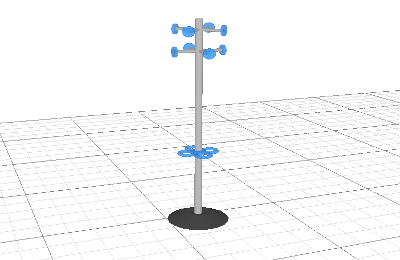
\includegraphics[width=5.5cm]{images/hanger} &
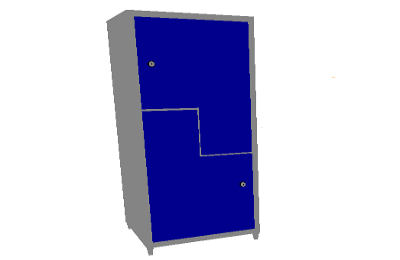
\includegraphics[width=5.5cm]{images/wardrobe} \\
 (a) & (b) \\
\end{tabular}
\begin{tabular}{c @{\hspace{1em}} c}
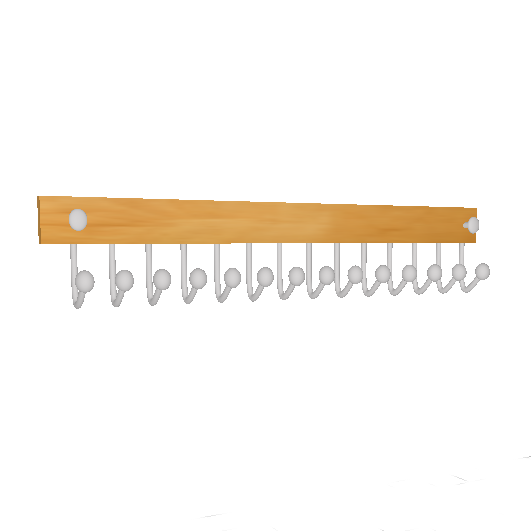
\includegraphics[width=5.5cm]{images/attaccapanni2} &
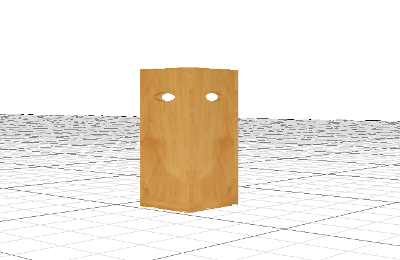
\includegraphics[width=5.5cm]{images/portaombrelli} \\
 (c) & (d) \\
\end{tabular}
\end{center}
\caption{Dettaglio Plugin: (a) appendiabiti, (b) armadietto, (c) attaccapanni, (d) portaombrelli}\label{fig:figura1}
\end{figure}
\newpage

Il secondo gruppo di \emph{Plugin} riportato sono (Figura~\ref{fig:figura2}) è composto dal mobilio classico
prensente in aula scolastica: un banco, una cattedra, una lavagna ed una lavagna interattiva multimediale (lim).\\

\begin{figure}[htbp]
\begin{center}
\begin{tabular}{c @{\hspace{1em}} c}
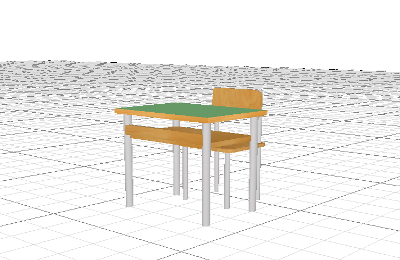
\includegraphics[width=5.5cm]{images/banco2} &
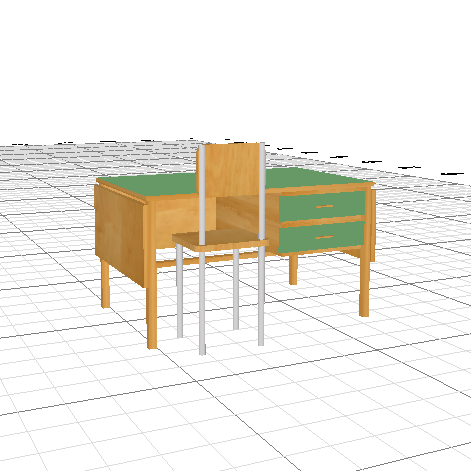
\includegraphics[width=5.5cm]{images/cattedra2} \\
 (a) & (b) \\
\end{tabular}
\begin{tabular}{c @{\hspace{1em}} c}
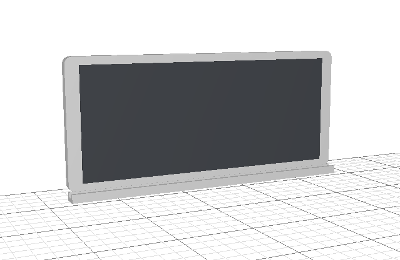
\includegraphics[width=5.5cm]{images/lavagna} &

\includegraphics[width=5.5cm]{images/lim} \\
 (c) & (d) \\
\end{tabular}
\end{center}
\caption{Dettaglio Plugin: (a) banco, (b) cattedra, (c) lavagna, (d) lim}\label{fig:figura2}
\end{figure}
\newpage

Il terzo gruppo di \emph{Plugin} è importante per quanto riguarda la tematica del rispetto dell'ambiente ed ecologia.
Come si vede in Figura~\ref{fig:figura3} sono presenti: un cestino, un gruppo di cestini
per la raccolta differenziata, un condizionatore d'aria ed un termosifone.\\


\begin{figure}[htbp]
\begin{center}
\begin{tabular}{c @{\hspace{1em}} c}
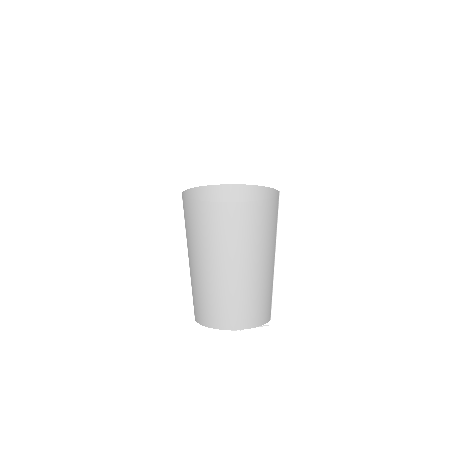
\includegraphics[width=5.5cm]{images/cestino} &
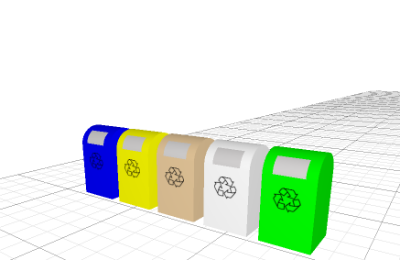
\includegraphics[width=5.5cm]{images/recycling-bins} \\
 (a) & (b) \\
\end{tabular}
\begin{tabular}{c @{\hspace{1em}} c}
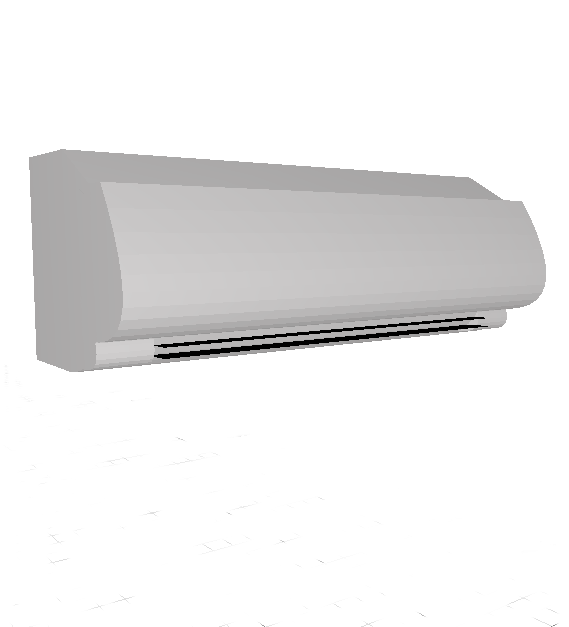
\includegraphics[width=5.5cm]{images/condizionatore} &
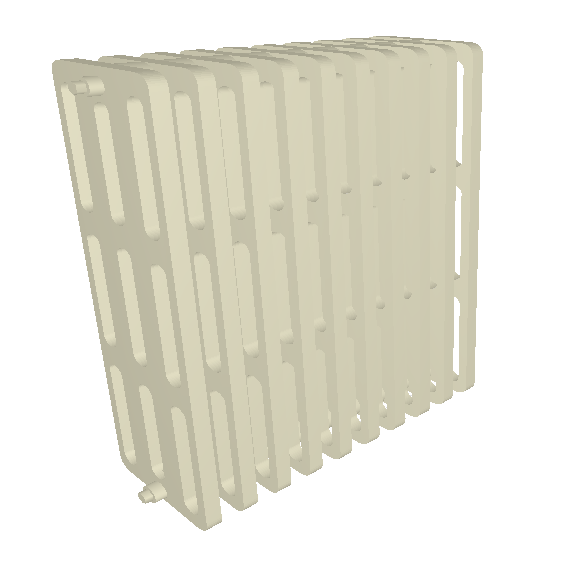
\includegraphics[width=5.5cm]{images/termosifone} \\
 (c) & (d) \\
\end{tabular}
\end{center}
\caption{Dettaglio Plugin: (a) cestino, (b) cestini differenziata, (c) condizionatore, (d) termosifone}\label{fig:figura3}
\end{figure}
\newpage

Il quarto gruppo di plugin riportato sono (Figura~\ref{fig:figura4}): una libreria, un computer,
una finestra con tenda ed una con veneziana.\\

\begin{figure}[htbp]
\begin{center}
\begin{tabular}{c @{\hspace{1em}} c}
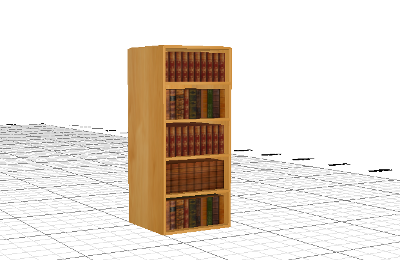
\includegraphics[width=5.5cm]{images/bookcase} &
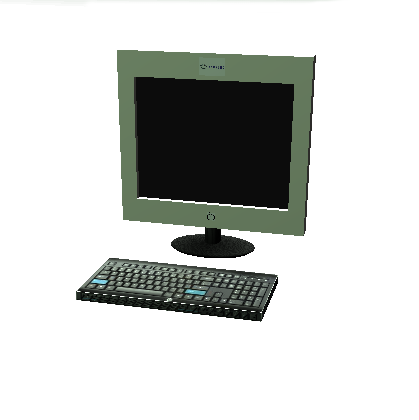
\includegraphics[width=5.5cm]{images/monitorPC} \\
 (a) & (b) \\
\end{tabular}
\begin{tabular}{c @{\hspace{1em}} c}
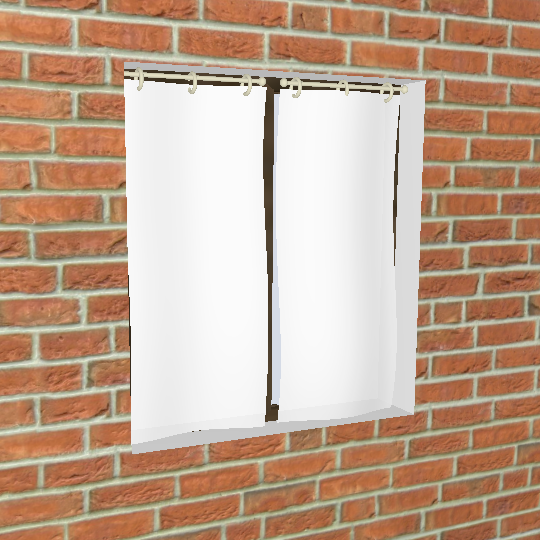
\includegraphics[width=5.5cm]{images/tenda} &
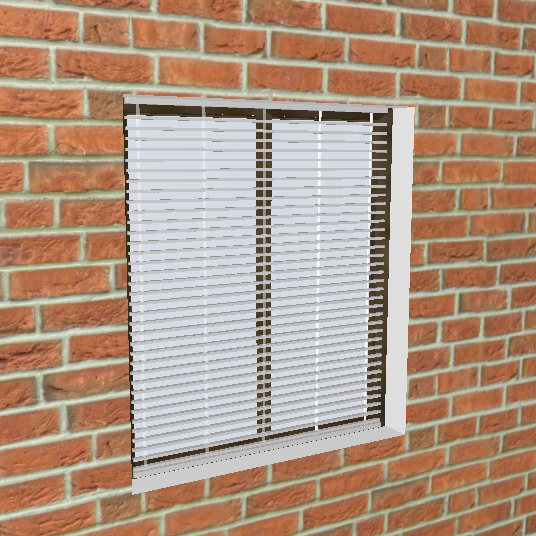
\includegraphics[width=5.5cm]{images/veneziana} \\
 (c) & (d) \\
\end{tabular}
\end{center}
\caption{Dettaglio Plugin: (a) libreria, (b) computer, (c) finestra con tenda, (d) finestra con veneziana}\label{fig:figura4}
\end{figure}

\newpage
